\chapter{Literature Review}
\label{chapter: 2}

This chapter provides an in depth look into technical solutions for the problems that the project will tackle, divided into three key areas: ball position, ball velocity and ball trajectory. The primary source for this research is from papers written by past participants in the RoboCup competition. 

\section{Measuring Ball Position}

\subsection{Camera Calibration}

Camera calibration (specifically geometric camera calibration) is the process of estimating the parameters of a camera to remove distortions from the images it captures. A camera has two types of parameters that can be estimated: intrinsic and extrinsic. Hartley and Zisserman \cite{Hartley2004} describe these parameters.

Extrinsic parameters define the transformation between 3D world coordinates and 3D camera coordinates. This includes a rotation $R$ and a translation $T$. 

The intrinsic parameters for a camera are its focal length in pixels $(f_x, f_y)$, its optical centre in pixels $(c_x, c_y)$ and the skew coefficient between the x and y axes $s$, although this is often zero. The parameters can be summarised in the camera intrinsic matrix $K$:

\[ K = 
\begin{bmatrix}
f_x & s & c_x\\
0 & f_y & c_x\\
0 & 0 & 1
\end{bmatrix}
\]

The output of a camera may also be affected by lens distortion. The first type of lens distortion is radial distortion which can cause straight lines to appear curved. It can be represented as follows:

\[ x_{distorted} = x(1+k_1 r^2 + k_2 r^4 + k_3 r^6) \]
\[ y_{distorted} = y(1+k_1 r^2 + k_2 r^4 + k_3 r^6) \]

\noindent where $x, y$ are the undistorted pixel positions, $k_1, k_2, k_3$ are the radial distortion coefficients and $r^2 = x^2 + y^2$.

The other type of lens distortion is tangential distortion which causes some parts of the image to appear closer than they should be. It can be represented as follows: 

\[ x_{distorted} = x + [2 p_1 x y + p_2(r^2 + 2 x^2)] \]
\[ y_{distorted} = y +[p_1 (r^2 + 2 y^2) + 2 p_2 x y] \]

\noindent where $x, y$ are the undistorted pixel positions, $p_1, p_2$ are the tangential distortion coefficients and $r^2 = x^2 + y^2$.

The five parameters that need to be estimated are given by:

\[ \text{Distortion coefficients} = (k_1, k_2, p_1, p_2, k_3) \] 

\nocite{Zhang2000}
\nocite{Heikkila1997}
\nocite{Ling2019}

\subsection{Non-Neural Object Detection}

Object detection is a type of computer vision problem that attempts to find instances of an object class in an image. In this case the problem is specific to finding the location of a single ball in an image. One approach to this problem is the non-neural approach, in which various types of algorithms must be combined to find these instances. 

Feature extraction algorithms aim to reduce the complexity of some data by picking out only the relevant features. In the field of computer vision this involves finding relevant areas of interest in an image. 

Feature descriptors take an image and output a feature vector, which is a representation of the original image in a format that can more easily be processed by models such as classifiers. 

A classifier is a model that can assign an output value to a given input feature vector. This project only looks at binary classifiers, in which the output is either true or false. Many classifiers are trained using supervised learning, which is a type of machine learning algorithm that learns how to map the input to output from a dataset of labelled input-output pairs. 

\subsubsection{Circular Hough Transform}

The Hough transform is a feature extraction algorithm originally designed to detect lines in an image, which has since been extended to detect arbitrary shapes. To identify the position of a ball, the circular Hough transform is useful. The first step is to apply an edge detection operator, for example the Sobel or Canny edge detectors. Next the parameter space must be decided. 

\[ r^2 = (x-a)^2 + (y-b)^2 \]

For a circle with a known radius \textit{r}, the search for the centre \textit{(a, b)} can be conducted in 2D parameter space. If the radius is unknown a 3D parameter space is required as the radius must also be searched for. Now the voting procedure can take place, resulting in an accumulator where each point in the parameter space is assigned a value by the Hough transform. The coordinates of the peaks in the accumulator correspond to the attributes of the circles found in the image \cite{ribeiro2009}.

The performance of the algorithm could be improved by first applying a colour segmentation to the image \cite{jonker}. False positives could be removed by validating the results. A distance-dependant threshold could be introduced, so closer candidates require a larger value for their local maximum to be included. Another validation could be checking that the sum of all floor coloured pixels in a bounding box drawn around the candidate is not too large \cite{cambada}.

\subsubsection{Colour Image Segmentation}

Image segmentation is the process of breaking down an image into various segments to make analysis easier. Colour segmentation uses the colour information of the image to create these segments. First the colour space must be chosen, for example RGB, HSV or YUV. Colour classes are then chosen as ranges inside this colour space and stored in a lookup table. HSV is the easiest to calibrate colour classes for, due to the colour information being limited to only the hue channel. Colour classes can be calibrated manually by a human, although this is tedious and not robust to changes in lighting. Automatic on-line calibration \cite{Guerrero2008} could be used instead to provide better results.

A simple method of segmenting the image is to calculate the colour class of each pixel individually according to the lookup table, but a more sophisticated technique such as colour region growing \cite{Gunnarsson2006} can achieve better results.

\subsubsection{K-Means Clustering}

K-means clustering aims to cluster data into k clusters, where each data point belongs to the cluster with the nearest mean. The problem is NP-hard but Hartigan and Wong\cite{Hartigan1979} present an efficient algorithm, that aims to find local optima rather than a perfect solution.

In image processing, k-means clustering can be used to find what colours are in an image, and which colours are the most dominant. The most important parameter is k, too few clusters could mean that different colours are included in the same cluster whereas too many clusters could mean that one colours is separated into multiple clusters.

\begin{figure}[ht]
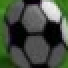
\includegraphics[width=3cm]{images/kmeans_ball.png}

\includegraphics[width=3cm]{images/kmeans_palette.png}
\centering
\caption{An example of using k-means clustering to find the dominant colours in an image}
\end{figure}

\subsubsection{Histogram of Oriented Gradients}

The histogram of oriented gradients (HOG) is a method of feature description, meaning that it summarises interesting information about an image into a feature vector. The algorithm breaks the image down into smaller cells and analyses the edge directions in these cells, building a histogram of gradient directions. The implementation of the algorithm as described by Dalal and Triggs \cite{Dalal2005} is outlined below:

\begin{enumerate}
    \item Gradient Computation
    
    Dalal and Triggs discuss preprocessing in the form of gamma/ colour normalisation, but find that it has little effect, possibly due to the normalisation in later steps achieving the same results. The first step is therefore to calculate the gradient values in both the horizontal and vertical directions. Dalal and Triggs suggest to use the following filter kernels:
    \[ [-1, 0, 1] \text{ and } [-1, 0, 1]^T \]
    
    
    \begin{figure}[H]
        \caption{An example of gradient computation}
        \centering
        \begin{tikzpicture}
        \draw[xstep=0.75cm,ystep=0.5,color=gray] (0,0) grid (2.25,1.5);
        \matrix[matrix of nodes,
        inner sep=0pt,
        anchor=south west,
        nodes={inner sep=0pt,text width=.75cm,align=center,minimum height=.5cm}
        ]{
        75 & 14 & 61 \\
        187 & 90 & 129 \\
        93 & 146 & 3 \\
        };
        \end{tikzpicture}
        
        The gradients at the centre pixel are:
        
        Gradient in x direction = $129 - 187 = -58$
        
        Gradient in y direction = $146 - 14 = 132$
    \end{figure}
    
    
    \item Spatial/ Orientation Binning
    
    The next step is to compile these gradients into a histogram. The image is broken down into cells, each of which has a set of orientation bins. These bins are evenly spaced over the range 0\degree - 180\degree for an unsigned gradient. Dalal and Triggs find that using any more than 9 bins has little difference on performance. Each pixel calculates a weighted vote using the orientation and magnitude of the gradient at that point, which is accumulated into the orientation bins for that cell.
    
    \begin{figure}[H]
        \caption{An example for HOG orientation binning}
        \centering
        The orientation at the centre pixel can be calculated by $atan(\frac{132}{-58}) = -66.28\degree$
        
        As an unsigned orientation $-66.28\degree + 180\degree = 133.72\degree$
        
        Assuming a magnitude of 100, this orientation is inserted into a blank set of orientation bins.
        
        \[100 * \frac{13.72}{20} = 68.6, 100 * \frac{6.28}{20} = 31.4 \]
        
        \begin{tikzpicture}
        \draw[xstep=1cm,ystep=0.5,color=gray] (0,0) grid (9,1);
        \matrix[matrix of nodes,
        inner sep=0pt,
        anchor=south west,
        nodes={inner sep=0pt,text width=1cm,align=center,minimum height=.5cm}
        ]{
         \textbf{0\degree} & \textbf{20\degree} & \textbf{40\degree} & \textbf{60\degree} & \textbf{80\degree} & \textbf{100\degree} & \textbf{120\degree} & \textbf{140\degree} & \textbf{160\degree} \\
         0 & 0 & 0 & 0 & 0 & 0 & 68.6 & 31.4 & 0 \\
        };
        \end{tikzpicture}
    \end{figure}
    
    \item Normalisation and Descriptor Blocks
    
    Local normalisation is used to reduce the effect of variations in illumination and contrast. Cells are grouped into larger blocks, which typically overlap. The normalisation is then calculated over these blocks. Dalal and Triggs evaluate two classes of block geometries, rectangular (R-HOG) and circular (C-HOG). They found that the optimal configuration for R-HOG is for blocks to be made up of 4 cells in a square. 
    
    Dalal and Triggs describe four block normalisation methods. Let \textbf{v} be the unnormalised descriptor vector, $||\textbf{v}||_k$ be its \textit{k}-norm  for \textit{k} = 1,2, and $\epsilon$ be a small constant. 
    \[ \text{L2-norm: } \textbf{v} = \frac{\textbf{v}}{\sqrt{||\textbf{v}||^2_2 + \epsilon^2}} \]
    L2-Hys: L2-norm followed by clipping (limiting the maximum values of \textbf{v} to 0.2) and renormalising
    \[ \text{L1-norm: } \textbf{v} = \frac{\textbf{v}}{||\textbf{v}_1|| + \epsilon} \]
    \[ \text{L1-sqrt: } \textbf{v} = \sqrt{\frac{\textbf{v}}{||\textbf{v}_1|| + \epsilon}} \]
    
\end{enumerate}


\begin{figure}[ht]
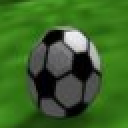
\includegraphics[width=3cm]{images/hog_ball.png}
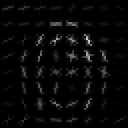
\includegraphics[width=3cm]{images/hog.png}
\centering
\caption{A visualisation of the HOG descriptor}
\end{figure}

Farazi et al. \cite{Farazi2016} use a HOG descriptor for a cascade classifier, trained using the AdaBoost technique to reject false positives from a list of ball candidates. As the HOG descriptor is not rotation invariant, for each positive sample in their dataset they add samples rotated by 10\degree, 20\degree and mirrored horizontally. The rotations are limited to this amount to allow the classifier to learn the shadow under the ball.

\subsubsection{Support-Vector Machine Classifier}

The support-vector machine is a supervised learning model for the two-group classification problem. The algorithm was developed by Cortes and Vapnik\cite{Cortes1995}. The goal of the machine is to find the hyperplane that separates the two classes while having the largest distance to the nearest data point of either class. However, there is often not a linear solution in the original dimensional space. To solve this, the data is be mapped to a higher-dimensional space, for which a linear solution does exist. This process is optimised by ensuring that the dot product can be used to transform hyperplanes between these dimensional spaces.

\begin{figure}[H]
    \centering
    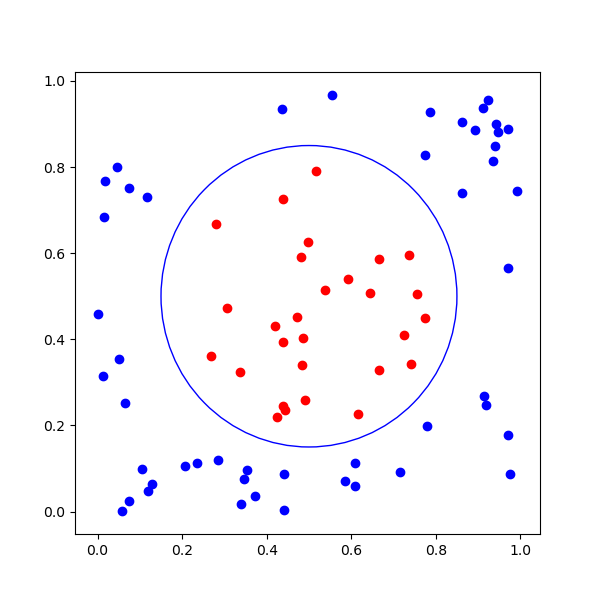
\includegraphics[width=5cm]{images/svm1.png}
    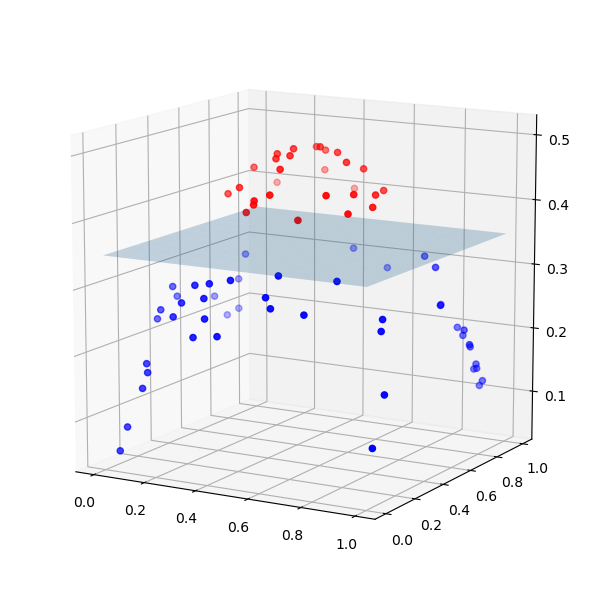
\includegraphics[width=5cm]{images/svm2.png}
    \caption{An illustration of an SVM mapping to a higher dimensional space}
    \centering
\end{figure}

Menashe et al. \cite{Menashe2017} compare the SVM to simple deep neural network (DNN) models for ball classification in RoboCup. They find that both methods have high accuracy, although the DNNs have a higher recall. The generalisation of the models is also tested, with the SVM producing much worse results for a different dataset. This highlights the importance of training the classifier on a dataset which is representative of the situations that could occur in a real game. 

\subsubsection{Ensemble Learning and AdaBoost}

In ensemble learning, a classifier is formed by combining multiple less accurate algorithms. An ensemble is guaranteed to be more accurate than any of its individual members if each classifier is accurate (better than random guessing) and diverse (makes different errors on new data points). Dietterich\cite{Dietterich2000} compares various methods of constructing ensembles, and concludes that AdaBoost is the most effective.

AdaBoost (short for adaptive boosting) is a type of boosting algorithm introduced by Freund and Schapire\cite{Freund1996}. The algorithm builds an ensemble classifier by training subsequent models to correct the mistakes of previous model. This is achieved by assigning a weight to each sample in the training data, and increasing these weights for samples which have previously been misclassified.

\subsection{Neural Object Detection}

The neural approach to object detection produces results directly from an input image, without any intervening algorithms, at the cost of increased computational complexity. The primary method for this the the convolutional neural network.

\subsubsection{Convolutional Neural Network}

A artificial neural network (ANN) is a computational model that is made up of a series of connected neurons, much like the human brain. Traditional ANNs are not suitable for image processing due to the computational complexity of the number of connections required. A convolutional neural network (CNN) is a class of ANN that uses convolutional layers to reduce the number of connections between layers, thus making them effective in processing images.

Convolutional layers learn kernels as parameters. Kernels are matrices that are convolved across the width and height of the input to produce an activation map. The activation maps for each kernel are stacked together to produce the layer's output. Convolutional layers have three hyperparameters, depth, stride and padding. The depth refers to the number of neurons in a layer that connect to the same region of the input. The stride sets how many pixels kernels should move at a time, and can cause overlapping between regions. Padding controls how many pixels should be added to the border of the output, this is commonly used to preserve the size exact size of the input.

Pooling layers are used for dimensionality reduction, decreasing the computation power needed to process the layer. The most common type is max pooling, where the image is broken down into smaller regions and only the maximum value is taken from each. 

Fully connected layers are used at the end of the network for classification \cite{cnn}.

In RoboCup various approaches have been taken for classification of the ball position. One method is to break the image down into smaller "patches" and evaluate each patch between two classes: ball or no ball. This has the advantage a large quantity of training data is easier to produce, however each patch does not have any further context about the image which can make classification more difficult \cite{Gabel2018}. Alternatively the network could be trained to estimate a 2D normal distribution of the ball's position, where the distortion of the distribution also gives an idea of how noisy the image is \cite{Speck2016}. Another method is to have the output be a low resolution heatmap of the original image, which can achieve pixel level accuracy of the ball's position \cite{Speck2018}.

\nocite{Kukleva2019}
\nocite{Teimouri2019}

\subsection{Sensor Fusion}

Sensor fusion is the process of combining sensory data from various sources in order to reduce uncertainty. In the case of a team based problem such as robot football, local sensor fusion and global sensor fusion can be distinguished between. Local sensor fusion refers to data from several sensors on one robot being combined, whereas in global sensor fusion data from different robots is combined. 

One method of global sensor fusion is to calculate the arithmetic mean of all reported values. This is simple however it is not very accurate as one incorrect reading will significantly affect the estimate. This problem can be mitigated somewhat by weighting values based on their distance to the ball, as closer readings are more likely to be accurate however this does not completely solve the problem. Various other methods such as Monte Carlo Localisation or a Kalman filter can be used to achieve more accurate results (\cite{Ferrein2005}).

\subsubsection{Kalman Filter}

The Kalman filter is a local sensor fusion algorithm that combines sensor measurements with predictions from a dynamic model to produce a more accurate reading than the measurements alone, by estimating a joint probability distribution over these variables. The Kalman filter runs in real-time, producing an estimate at each timestep from only the last reading and the current sensor measurements.

The following matrices must be specified:
\begin{itemize}
    \item $F_k$, the state-transition model
    
    Transforms a state to the state at the next timestep, according to the laws of physics.
    \item $H_k$, the observation model
    
    Maps the state to only the values that should be observed.
    \item $Q_k$, the covariance of the process noise
    
    Covariance applied to the predicted state.
    \item $R_k$, the covariance of the observation noise
    
    Covariance applied to the observed state.
    \item Optionally $B_k$, the control-input model
    
    Applied to the control vector $u_k$
\end{itemize}

The following matrices are calculated at each timestep.
\begin{itemize}
    \item $\hat{x}_{j|k}$, state estimate at time j given observations up to and including at time k
    \item $P_{j|k}$, estimated covariance matrix at time j given observations up to and including at time k
    \item $K_k$, Kalman gain at time k
    \item $z_k$, a measurement of the true state, $x_k$ using $H_k$ and $R_k$
\end{itemize}


During each timestep k, the Kalman filter has two phases: predict and update. At the predict phase, the Kalman filter calculates the estimated state and covariance using the previous state and covariance as well as the state-transition model and the process noise. The current measurements are supplied to the update phase, during which the estimated state and covariance are updated, taking into account the observation model and the observation covariance.

Equations for the prediction step:

\[ \hat{x}_{k|k-1} = F_k \hat{x}_{k-1|k-1} + B_k u_k  \] 
\[ P_{k|k-1} = F_k P_{k-1|k-1} F^T_k + Q_k \]

Equations for the update step:

\[ K_k = P_{k|k-1} H^T_k(H_k P_k H^T_k + R_k)^{-1} \]
\[ \hat{x}_{k|k} = \hat{x}_{k|k-1} + K_k(z_k - H_k \hat{x}_{k|k-1}) \]
\[ P_{k|k} = P_{k|k-1} - K_k H_k P_{k|k-1} \]

\nocite{Lauer2005}

\section{Measuring Ball Velocity}

\subsection{Linear Regression}

It is necessary to estimate the current velocity of the ball before any prediction about its future trajectory can be made. Silva et al. \cite{Silva2010} discussed various methods of calculating this velocity. The first is to calculate the instant velocity, by taking the change in position over the delta time, however this is not very accurate as it is heavily affected by noise. Another approach is to use the velocity calculated by the Kalman filter. This creates a smooth estimate of the velocity however it is slow to react to change, making it inappropriate for the dynamic world of robot football. The method used by Silva et al. is linear regression \cite{Motulsky2011}. 

A buffer of the last n positions is kept, over which a regression line can be calculated. To allow the regression to converge more quickly, the older values are removed from the buffer whenever a change in velocity is detected.

\subsection{Exponentially Weighted Moving Average}

The exponentially weighted moving average (EWMA) is a method of calculating a moving average, where the weighting factors decrease exponentially. This means that more recent values have more influence on the final average, which would be useful in calculating the changing velocity of a ball. The EWMA for a series Y can be calculated recursively:

\[ S_t = \begin{cases}
    Y_1, & t = 0 \\
    \alpha Y_t + (1-\alpha)S_{t-1}, & t > 0 \\
\end{cases}\]

\noindent where $\alpha$ is a constant smoothing factor between 0 and 1, $Y_t$ is the series value at time $t$ and $S_t$ is the EWMA at time $t$.

\section{Predicting Ball Trajectory}
\label{section: trajectory lit review}

Yazdankhoo et al. \cite{Yazdankhoo2018} compare various methods of predicting ball trajectory, assuming that the ball does not leave the ground. A distinction can be made between online and offline methods. In online methods, the trajectory is predicted as the ball moves without any prior knowledge of the environment whereas in  offline methods, information about the environment is learnt beforehand. 

\subsection{Online methods}

\subsubsection{Double Exponential Smoothing}

Exponential smoothing is a method for smoothing time series data (a series of data points indexed by time). Double exponential smoothing (DES) is an application of this which accounts for trends in the data. Assuming $x$ is the position of the ball at time $t$:

\[ S_i = \alpha x_i + (1 - \alpha) (S_{i-1} + b_{i-1}) \]
\[ b_i = \gamma(S_i - S_{i-1}) + (1 - \gamma)b_{i-1} \]

\noindent where  $0 < \alpha, \gamma \leq 1$, $i = 1,2,...,n$. $S_i$ and $b_i$ are calculated in $n$ steps. The predicted position $\hat{x}$ is calculated by:

\[ \hat{x}_{n + m} = s_n + m b_n \]

$\alpha$ and $\gamma$ must be estimated in some way, either as constants or using some adaptive technique.

\subsubsection{Autoregressive Method}

An autoregressive (AR) model is a representation of a random process. The prediction of a variable depends linearly on its previous values and a random process such as white noise. In the case of ball trajectory this randomness accounts for noise and inaccuracies of the system. 

\subsubsection{Quadratic Prediction}

Quadratic prediction (QP) uses the laws of physics to predict a ball trajectory. If we assume that friction is the only force acting on the ball, then its motion can be represented by the following kinematic equation:

\[ x = \frac{1}{2}at^2 + v_0t + x_0 \]

where \textit{a} is the acceleration, \textit{$v_0$} is the initial velocity, \textit{$x_0$} is the initial position and \textit{t} represents time.

\textit{a}, \textit{$v_0$} and \textit{$x_0$} are all constants, and can all be calculated after three readings of the position of the ball have been made.

\subsection{Offline Methods}

\subsubsection{Self-Perturbing Recursive Least Squares}

Self-perturbing recursive least squares\cite{Park1992} (SPRLS) is an algorithm that recursively determines the parameters of a system. 

\[ L_i = \frac{P_{i-1} \phi_i}{1 + \phi^T_i P_{i-1} \phi_i} \]
\[ P_i = P_{i-1}(I - L_i \phi^T_i) + \beta NINT(\lambda e^2_{i-1})I \]
\[ \hat{\theta}_i = \hat{\theta}_{i-1} + L_i(y_i - \phi^T_i \hat{\theta}_{i-1}) \]

\noindent where $e = y - \hat{y}$ is the estimation error, $y = \theta^T \phi$ and $\hat{theta}^T \phi$ are real and estimated outputs respectively, $\phi$ is the vector of input parameters, $\theta$ is the vector of estimated parameters, $I$ is the identity matrix, $\beta$ is the design coefficient, $\lambda$ is the sensitivity coefficient and $NINT$ is defined as:

\[ NINT(x) = \begin{cases}
    x, & x \leq 0.5 \\
    0, & 0 \leq x < 0.5
\end{cases}
\]

Using the kinematic equations from quadratic prediction:

\[ -2(x - v_0 t - x_0) = \mu g t^2 \]

Comparing with $y = \theta^T \phi$:

\[ y = -2(x - v_0 t - x_0) \]
\[ \theta^T = \mu g \]
\[ \phi = t^2 \]

\subsection{Combining Offline and Online Methods}

In a later paper Yazdankhoo et al. \cite{Yazdankhoo2021} propose a trajectory prediction method combining both online and offline methods. For the offline part, a k-nearest neighbour regression, while an autoregressive method is used for the online portion. The results of these two algorithms are combined according to a weighting coefficient $\alpha$. Rather than updating the trajectory every timestep, updates are limited to instances when the ball movement changes unexpectedly. 

\nocite{Maire2000}
